\documentclass[12pt]{article} % The document class with options

\usepackage[margin=1in]{geometry}
\usepackage[utf8]{inputenc} 
\geometry{a4paper}
\usepackage{newtxtext,newtxmath}
\usepackage[T1]{fontenc}
\usepackage{amsmath} % for advanced math typesetting
\usepackage{amsfonts}
\usepackage{microtype}
\usepackage{graphicx}

\begin{document}
\setlength{\parskip}{1em} 
\setlength{\parindent}{0pt}
\newcommand{\vect}[1]{\mathbf{#1}}

\begin{titlepage}  % This starts a title page environment
    \centering    % Center everything on the page

    %--- Add space at the top of the page ---
    \vspace*{2cm}
    
    %--- Title ---
    \normalsize \textbf{MATH 521 Project Report} \\
    \vspace{0.5cm}  % Space between lines
    \normalsize\textbf{A Comprehensive Review of Weak Galerkin Finite Element Method for Second-Order Elliptic Problems and N-S Equations} \\
    \vspace{2cm}  % Space between the title and the author name
    
    %--- Author ---
    \normalsize by\\
    \vspace{1cm}
    \normalsize Jincong Li \\ 
    \vspace{1cm}
    \normalsize M.Eng, The University of British Columbia, 2024
    \vspace{11cm}  % Space between the author and the date
    
    %--- Date ---
    \normalsize \today

    \vfill  % Push the following content to the bottom of the page
    %--- Bottom part of the page ---
    © Jincong Li, 2024
\end{titlepage}
\tableofcontents
\newpage
\section{Abstract}
This report presents a comprehensive examination of the Weak Galerkin (WG) Finite Element Method (FEM), a novel numerical approach designed for the solution of second-order elliptic problems and Navier-Stokes equations. The WG method, which incorporates the concept of weak gradients, offers significant advantages in terms of flexibility and applicability to discontinuous functions. It extends traditional FEM by allowing for the inclusion of discontinuous polynomial spaces and enhances the method's ability to handle complex geometrical and boundary conditions. The primary focus of this review is to validate the theoretical aspects of the WG method through rigorous error analysis and to demonstrate its effectiveness via numerical examples. The convergence behavior of the WG method is thoroughly discussed, with particular attention to its performance in maintaining high accuracy and adherence to physical conservation laws.
\section{Introduction}
\subsection{Overview of Numerical Methods}
Existing finite element methods are generally classified into two main groups: 
\begin{enumerate}
    \item Methods that focus on the main variable \( u \), and 
    \item Methods that consider both \( u \) and auxiliary variables
\end{enumerate}
The first category focus on approximating the solution u of the PDE directly, such as the Standard Galerkin FEM \cite{Ciarlet1978} which 
use variational principles to approximate the solution u by minimizing an energy functional.
It typically requires the solution space to be a subset of the Sobolev space $H^1$. Another example is the Interior Penalty Type Discontinuous 
Galerkin Methods\cite{Riviere1999}: These are a class of Galerkin methods that allow 
for discontinuities in the solution across the boundaries of the elements in the discretized domain. 
They are particularly useful for dealing with high-contrast media or when higher-order polynomials 
are used for the approximation. The method involves adding penalty terms to the formulation to 
enforce continuity constraints weakly.

The second category involve formulating the PDE problem by introducing auxiliary variables, 
typically representing physical quantities like flux, and then seeking solutions for
both the primary variable u and the auxiliary variable(s). This approach can lead to 
systems of equations that capture more physical properties directly, such as conservation 
laws. One example is the Standard Mixed Finite Elements\cite{Raviart1977}. This approach 
is beneficial for problems where maintaining local conservation laws is important. Another example is the Various Discontinuous Galerkin Methods Based on Both Variables\cite{Jeon2010}: These methods extend 
the discontinuous Galerkin framework to handle both the primary variable and auxiliary 
variables. Notice that this approach combines the advantages of discontinuous Galerkin 
methods (such as flexibility in handling complex geometries and material discontinuities) 
with the ability to approximate additional physical quantities directly. 


The weak Galerkin finite element method, which will be reviewed later builds closely on the mixed finite element method, adopting ideas from Fraeijs 
de Veubeke \cite{Veubeke1965} and the hybridizable discontinuous Galerkin (HDG) method\cite{Cockburn2009}. 
Specifically, the weak Galerkin (WG) method is equaivalent to some of the regular mixed finite element methods and the HDG 
method under certain conditions (like \( b = 0, c = 0, \) and \( a \) is constant). However, the WG method is different from them when these 
coefficients are not constant. It introduces the concept of weak gradients, which gives us a systematic way to handle functions  
with discontinuities at the boundaries of domain pieces. This approach is really flexible and can be adapted to other kinds of 
differential equations that involve different types of differential operators, such as divergence and curl\cite{Wang2013}.



\section{Weak Galerkin Finite Element Method}
As discussed in the introduction section, The concept of weak gradients shall provide a systematic
framework for dealing with discontinuous functions defined on elements and their boundaries in a near classical sense\cite{Wang2013}. And following that, a second-order elliptic equation will be used as an example to show how the weak Galerkin method could be constructed in details.
\subsection{Weak Gradient Operator and Its Approximation}

This section introduces the weak gradient operator, which is tailored for a space of generalized functions. This operator will be used to discretize 
partial differential equations. Let \(K\) be any polygon-shaped domain with an interior, denoted \(K_0\), and a boundary, denoted \(\partial K\). 
In this domain, a weak function is a function \(v = \{v_0, v_b\}\) where \(v_0\) is in \(L^2(K)\), essentially, \(v_0\) describes how \(v\) behaves 
inside \(K\). And \(v_b\) is in \(H^{\frac{1}{2}}(\partial K)\), which defined as the value of \(v\) on the boundary of \(K\). 
Importantly, \(v_b\) might not directly relate to the trace of \(v_0\)\cite{Wang2013}. The space of these weak functions denoted as \(W(K)\), is defined by:

\begin{equation}
    W(K) = \left\{ v = \{v_0, v_b\} : v_0 \in L^2(K), v_b \in H^{\frac{1}{2}}(\partial K) \right\}.
\end{equation}

Notice that regarding this definition, special attention has been paid to the space that $v_b$ lives in, $H^{\frac{1}{2}}(\partial K)$. Normally, $H^{-\frac{1}{2}}(\partial K)$ is enough and why $H^{\frac{1}{2}}(\partial K)$ is chosen here is not clear at this point, which leads to future investigation.

By defining weak function, for any \(v \in W(K)\), the weak gradient \(v\), denoted \(\nabla_w v\), acts in the dual space of \(H(\text{div}, K)\). Note the definition of \(H(\text{div}, K)\) is not presented here, for more information, please refer to\cite{Hu2019}. The action of \(\nabla_w v\) on any test function \(q \in H(\text{div}, K)\) is defined as follows:

\begin{equation}
    (\nabla_w v, q) = -\int_K v_0 \nabla \cdot q \, dK + \int_{\partial K} v_b q \cdot n \, ds,
\end{equation}

where \(n\) is the outward unit vector normal to \(\partial K\). This formulation shows that \(\nabla_w v\) is well-defined since the right-hand side is a bounded linear functional over \(H(\text{div}, K)\).
Similar to the definition of the weak derivative covered by the course material: if the components of \(v\) are restrictions of some function \(u \in H^1(K)\) on \(K_0\) and \(\partial K\), then \(\nabla_w v\) equals the classical gradient \(\nabla u\).

A discrete version of the weak gradient operator is introduced here, \(\nabla_w\) within a polynomial subspace of \(H(\text{div}, K)\). Assume \(r\) is any non-negative integer, and let \(P_r(K)\) be the set of polynomials on \(K\) with a maximum degree of \(r\). Define \(V(K, r)\) as a subspace comprising vector-valued polynomials of degree \(r\). The discrete weak gradient operator, \(\nabla_{w,r}\), is uniquely determined by the equation:

\begin{equation}
    \int_K \nabla_{w,r} v \cdot q \, dK = -\int_K v_0 \nabla \cdot q \, dK + \int_{\partial K} v_b q \cdot n \, ds, \quad \forall q \in V(K, r).
\end{equation}

The discrete weak gradient, \(\nabla_{w,r}\), thus represents a Galerkin-type approximation to the weak gradient operator \(\nabla_w\) using the space \(V(K, r)\). 
%The classic gradient operator \(\nabla = (\partial_{x_1}, \partial_{x_2})\) is typically applied to sufficiently smooth functions. In contrast, the weak gradient operator allows us to differentiate functions that may not be continuous across the boundaries of the domain elements, accommodating generalized function forms in the computation.

\subsection{Weak Galerkin Finite Element Method}

To illustrate how the discrete weak gradient be used in constructing the weak Galerkin method,
a general second-order elliptic equation with Dirichlet boundary conditions considered here: Find an unknown function \( u = u(x) \) satisfying the following conditions within a domain \( \Omega \):
\begin{align}
    -\nabla \cdot (a \nabla u) + \nabla \cdot (bu) + cu &= f \quad \text{in } \Omega \\
    u &= g \quad \text{on } \partial \Omega
\end{align}
where \( \Omega \) is a polygonal or polyhedral domain in \( \mathbb{R}^d \) (with \( d = 2, 3 \)), \( a = (a_{ij}(x)) \) is a \( d \times d \) symmetric matrix-valued function belonging to \( [L^\infty(\Omega)]^{d^2} \), \( b = (b_i(x)) \) is a \( d \times 1 \) vector-valued function, and \( c = c(x) \) is a scalar function on \( \Omega \).

And, the standard weak formulation demands that \(u \in H^1(\Omega)\) such that \(u = g\) on \(\partial\Omega\) and satisfies the following condition:

\begin{equation}
    (a \nabla u, \nabla v) - (bu, \nabla v) + (cu, v) = (f, v) \quad \forall v \in H^1_0(\Omega).
\end{equation}

Consider \(\mathcal{T} \) as a regular triangular division of the domain \(\Omega\) with a specific mesh size \(h\). In line with the Galerkin procedure, the weak Galerkin method adheres to two key principles:
\begin{enumerate}
    \item Substitute \(H^1(\Omega)\) with a space of discrete weak functions defined over the finite element partition \(\mathcal{T}\) and the boundaries of its triangular elements.
    \item Replace the classical gradient operator with a discrete weak gradient operator \(\nabla_{w,r}\) for weak functions on each triangle \(T\).
\end{enumerate}

For each triangle \(T\) in \(\mathcal{T}\), denote by \(P_j(T_0)\) the polynomials on \(T_0\) of degree no more than \(j\), and by \(P_\ell(\partial T)\) the polynomials on \(\partial T\) of degree no more than \(\ell\). A discrete weak function \(v = \{v_0, v_b\}\) on \(T\) is thus defined where \(v_0 \in P_j(T_0)\) and \(v_b \in P_\ell(\partial T)\). Define this space as \(W(T, j, \ell)\):

\begin{equation}
    W(T, j, \ell) = \{v = \{v_0, v_b\} : v_0 \in P_j(T_0), v_b \in P_\ell(\partial T)\}.
\end{equation}

The corresponding finite element space is combining \(W(T, j, \ell)\) over all triangles \(T\) in \(\mathcal{T}\), defined as:

\begin{equation}
    S_h(j, \ell) = \{v = \{v_0, v_b\} : \{v_0, v_b\}|_T \in W(T, j, \ell), \forall T \in \mathcal{T}\}.
\end{equation}

Define \(S^0_h(j, \ell)\) as the subspace of \(S_h(j, \ell)\) with boundary values vanishing on \(\partial\Omega\):

\begin{equation}
    S^0_h(j, \ell) = \{v = \{v_0, v_b\} \in S_h(j, \ell), v_b|_{\partial T \cap \partial \Omega} = 0, \forall T \in \mathcal{T}\}.
\end{equation}

Based on equation (3), the discrete weak gradient of a function \(v = \{v_0, v_b\}\) in \(S_h(j, \ell)\) on each element \(T\) is given by:

\begin{equation}
    \int_T \nabla_{w,r}v \cdot q \, dT = -\int_T v_0 \nabla \cdot q \, dT + \int_{\partial T} v_b q \cdot n \, ds, \quad \forall q \in V(T, r).
\end{equation}

To facilitate computations, the bilinear form \(a(w, v)\) for any \(w, v \in S_h(j, \ell)\) is defined as:

\begin{equation}
    a(w, v) = \sum_{T \in \mathcal{T}} \left( \int_T a \nabla_{w,r} w \cdot \nabla_{w,r} v \, dT - \int_T b w_0 \cdot \nabla_{w,r} v \, dT + \int_\Omega c w_0 v_0 \, d\Omega \right).
\end{equation} 
Thus, for the general second-order elliptic equation described in (4)\&(5), the weak Galerkin method could be stated as:
seek \( u_h = \{u_0, u_b\} \in S_h(j, \ell) \) satisfying the following boundary condition and equation:
\begin{align}
    a(u_h, v) &= (f, v_0), \quad \forall v = \{v_0, v_b\} \in S^0_h(j, \ell), \\
    u_b &= Q_{bg} \text{ on } \partial \Omega,
\end{align}
where \( Q_{bg} \) is an approximation of the boundary value in the polynomial space \( P_{\ell}(\partial T \cap \partial \Omega) \). 

\section{Existence \& Uniqueness of Solution of WG Method}
This section will look into the proof of the existence and uniqueness of solution \(u_h\). However, the full procedure has been developed in \cite{Wang2013}, so the purpose of this section is not to go over all the details again but rather to clarify the key ideas.
One key observation here is that from (12), one can conclude the uniqueness is equivalent to existence for \(u_h\) since the number of unknowns is the same as the number of equations \cite{Wang2013}. To prove uniqueness, suppose \( u^{(1)}_h \) and \( u^{(2)}_h \) are two solutions of equation (4.6). Define \( e \) as the difference between these two solutions:
$e = u^{(1)}_h - u^{(2)}_h$, and show that \( e = 0 \). The theorem brought up in \cite{Wang2013} is presented here:

\textbf{Theorem 1}\cite{Wang2013} Assume that the dual of the equation(4)\&(5)
with homogeneous Dirichlet boundary conditions has \(H^{1+s}\)-regularity for some \(s \in (0, 1]\). Then, the weak Galerkin finite element method defined in equation (12) has a unique solution in the finite element spaces \(S_h(j, j+1)\) and \(S_h(j, j)\) provided that the mesh size \(h\) is sufficiently small.

The proof starts from following analogy of Gårding’s inequality:

Let \( S_h(j, \ell) \) be the weak finite element space defined in equation (8) and \( a(\cdot, \cdot) \) be the bilinear form given in equation (11). There exist positive constants \( K \) and \( \alpha_1 \) satisfying the inequality
\begin{equation}
    a(v, v) + K(v_0, v_0) \geq \alpha_1(\|\nabla_{w,r}v\|^2 + \|v_0\|^2),
\end{equation}
for all \( v \in S_h(j, \ell) \). Since $v$ is arbitrary, let $v = e$ and get:
\begin{equation}
    a(e, e) + K \|e_0\|^2 \geq \alpha_1 (\|\nabla_w e\|^2 + \|e_0\|^2).
\end{equation}
With the help from this lemma:
Let \( e = \{e_0, e_b\} \) be a discrete weak function in \( S^0_h(j, j+1) \) and other assumptions remain the same. Then, there exists a constant \( C \) such that
\begin{equation}
    \|e_0\| \leq C h^s \|\nabla_w e\|,
\end{equation}
provided that the mesh size \( h \) is sufficiently small.
The RHS of (15) could be bounded by 
\begin{equation}
    \alpha_1 (\|\nabla_w e\|^2 + \|e_0\|^2) \leq K C^2 h^{2s} \|\nabla_w e\|^2.
\end{equation}
And then choose the mesh size \( h \) sufficiently small so that:
\begin{equation}
    K C^2 h^{2s} \leq \frac{\alpha_1}{2}.
\end{equation}
This condition ensures that:
\begin{equation}
    \|\nabla_w e\|^2 + \|e_0\|^2 = 0,
\end{equation}
And finally, lemma: Consider any function \( v = \{v_0, v_b\} \) in \( W(T, j, j+1) \). Define the discrete weak gradient \( \nabla_{w,j+1}v \) on a triangle \( T \), with the space \( V(T, r) \) composed of vector-valued polynomials of degree \( j+1 \), i.e., 
\begin{equation}
    V(T, r) = [P_{j+1}(T)]^2.
\end{equation}
Then, the condition \( \nabla_{w,j+1}v = 0 \) holds true on \( T \) if and only if \( v \) is constant across \( T \), meaning both \( v_0 \) and \( v_b \) are constants.

This implies that \( e \) is zero everywhere, demonstrating that:
\begin{equation}
    u^{(1)}_h = u^{(2)}_h.
\end{equation}
Thus, the two solutions are identical, confirming the existence as well as the uniqueness of the solution $u_h$ in the finite element space.

\section{Error Analysis of Solution of WG Method}
This section will investigate the error estimate for the WG FEM, however, the full proof is too tedious to present in this work. Thus, only the results is declared below, and we shall see an example in the next section that confirms the result.

Assume that the dual of the problem defined by equations (4) \& (5) possesses \( H^{1+s} \) regularity and the exact solution \( u \) is sufficiently smooth such that 
\[ u \in H^{m+1}(\Omega) \] 

Then the error can be summarized as follows:
Under the same assumption, there exists a constant \( C \) such that
\begin{equation}
    \|u_h - Q_h u\| \leq C \left( h^{1+s} \|f - Q_0 f\| + h^{m+s} \|u\|_{m+1} \right), 
\end{equation}
for \( s \in (0, 1] \), \( m \in (0, j + 1] \), provided that the meshsize \( h \) is sufficiently small.

If the exact solution \( u \) of equations (4) \& (5) has \( H^{j+2} \) regularity, then from above we have that
\begin{equation}
    \|u_h - Q_h u\| \leq C \left( h^{1+s}h^j \|f\|_j + h^{j+s+1} \|u\|_{j+2} \right)
    \leq C h^{j+s+1} \left( \|f\|_j + \|u\|_{j+2} \right),
\end{equation}
for some \( 0 < s \leq 1 \), where \( s \) is a regularity index for the dual of equations (4) \& (5). In the case that the dual has full \( H^2 \) (i.e., \( s = 1 \)) regularity, one would arrive at
\begin{equation}
    \|u_h - Q_h u\| \leq C h^{j+2} \left( \|f\|_j + \|u\|_{j+2} \right).
\end{equation}

\section{Application to Navier-Stokes Equations}
In this section, some numerical results are presented to demonstrate the effectiveness of proposed WG scheme for
solving the NS equations. Two examples\cite{Hu2019} are considered, and they are described as following:

Example 1: Consider a domain \( \Omega = (0, 1)^2 \). The load term \( f \) is chosen such that the analytical solution \( u(x, y) \) is given by:
\begin{equation}
    u(x, y) = \frac{1}{2}
    \begin{pmatrix}
        \sin^2(2\pi x) \sin(2\pi y) \cos(2\pi y) \\
        -\sin^2(2\pi y) \sin(2\pi x) \cos(2\pi x)
    \end{pmatrix}
\end{equation}
and the pressure term \( p(x, y) \) is defined as:
\begin{equation}
    p(x, y) = \pi^2 \sin(2\pi x) \cos(2\pi y).
\end{equation}

Example 2:
Consider the domain \( \Omega = (0, 1)^2 \). The load term \( f \) is chosen to correspond with the analytical solution \( u(x, y) \) and pressure \( p(x, y) \), given by:
\begin{equation}
    u(x, y) = 
    \begin{pmatrix}
        0.1 x^2 (1 - x)^2 (4y^3 - 6y^2 + 2y) \\
        0.1 y^2 (1 - y)^2 (4x^3 - 6x^2 + 2x)
    \end{pmatrix}.\\
    p(x, y) = x^3 y^3 - \frac{1}{16}.
\end{equation}
Note that in this example, the velocity \( u \) is not divergence free.
Those two example cases are tested on two grids shown below:
\begin{figure}[ht]
    \centering
    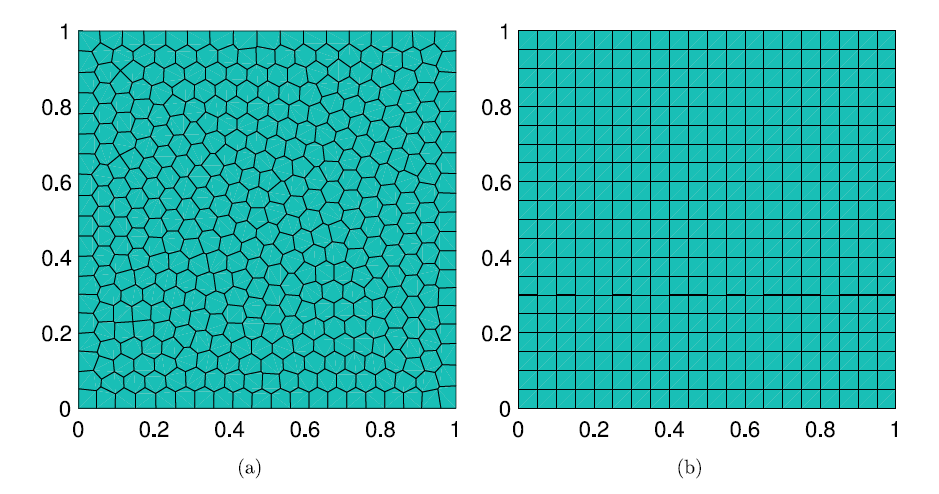
\includegraphics[width=1\textwidth]{NS_grid.png}
    \caption{(a) Polygonal mesh with h = 1/20; (b) Uniform rectangular mesh with h = 1/20.\cite{Hu2019}}
\end{figure}
\clearpage
The result of numerical tests are listed in the table below, and from which one could conclude that the \(H^1\)-error for velocity and the \(L^2\)-error for pressure exhibit convergence at the rate of \(O(h)\), which agrees the theorem 8.4. Additionally, the \(L^2\)-norm for velocity demonstrates a convergence rate of \(O(h^2)\), aligning with our expectations.
\begin{figure}[ht]
    \centering
    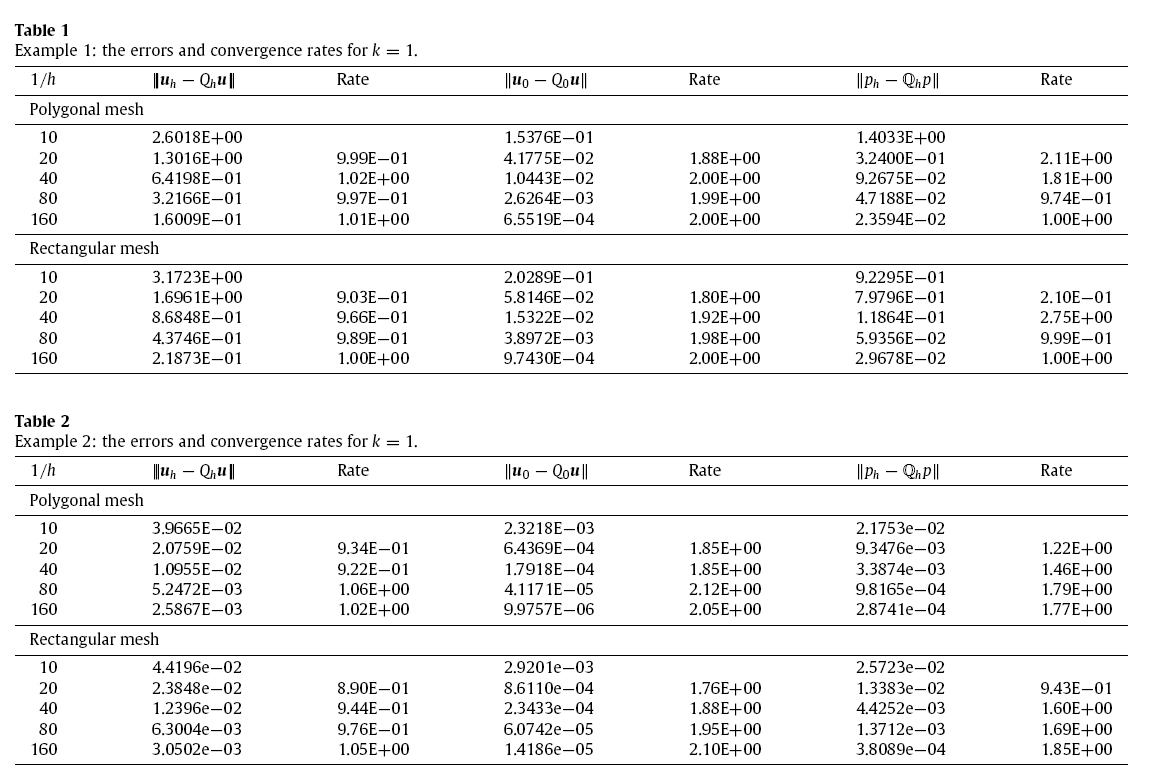
\includegraphics[width=1\textwidth]{NS_result.png}
    \caption{The errors and convergence rates for k = 1.\cite{Hu2019}}
\end{figure}
\clearpage
\section{Conclusion}
The investigation into the Weak Galerkin finite element method outlined in this report underscores its potential as a powerful tool for the numerical resolution of both elliptic and fluid dynamics problems. The method's robustness in handling complex problems with irregular geometries and discontinuous coefficients has been confirmed through both theoretical analysis and numerical testing. The convergence rates observed for the WG method align with the theoretical predictions, affirming its efficiency and accuracy. Future work may focus on extending the application range of the WG method to more complex multi-physics problems and exploring its integration with other numerical techniques to enhance computational performance. The ongoing development and refinement of the WG method will likely contribute significantly to the field of computational mathematics and engineering.

\section{Reference}
\begin{thebibliography}{99}

    \bibitem{Ciarlet1978}
    P.G. Ciarlet, \emph{The Finite Element Method for Elliptic Problems}, North-Holland, New York, 1978.
    
    \bibitem{Riviere1999}
    B. Riviere, M.F. Wheeler, V. Girault, \emph{Improved energy estimates for interior penalty, constrained and discontinuous Galerkin methods for elliptic problems. Part I}, Comput. Geosci., 8 (1999) 337--360.
    
    \bibitem{Raviart1977}
    P. Raviart, J. Thomas, \emph{A mixed finite element method for second order elliptic problems}, in: I. Galligani, E. Magenes (Eds.), Mathematical Aspects of the Finite Element Method, Lecture Notes in Math., vol. 606, Springer-Verlag, New York, 1977.
    
    \bibitem{Jeon2010}
    Y. Jeon, E. Park, \emph{A hybrid discontinuous Galerkin method for elliptic problems}, SIAM J. Numer. Anal. 48 (2010) 1968--1983.
    
    \bibitem{Cockburn2009}
    B. Cockburn, J. Gopalakrishnan, R. Lazarov, \emph{Unified hybridization of discontinuous Galerkin, mixed and continuous Galerkin methods for second-order elliptic problems}, SIAM J. Numer. Anal. 47 (2009) 1319--1365.

    \bibitem{Veubeke1965}
    B.X. Fraeijs de Veubeke, \emph{Displacement and equilibrium models in the finite element method}, in: O.C. Zienkiewicz, G. Holister (Eds.), Stress Analysis, John Wiley, New York, 1965.
    
    \bibitem{Wang2013}
    J. Wang, X. Ye, \emph{A weak Galerkin finite element method for second-order elliptic problems}, J. Comput. Appl. Math. 241 (2013) 103--115.
    
    \bibitem{Hu2019}
    Hu, X., Mu, L., \& Ye, X. (2019). \emph{A weak Galerkin finite element method for the Navier–Stokes equations}. Journal of Computational and Applied Mathematics, 362, 614--625. doi:10.1016/j.cam.2018.08.022
    
    \end{thebibliography}

\end{document}